\documentclass[a4paper]{article}

\usepackage{hyperref}

\author{Kerry Zhang 2014403073, Richard Luong 2014403075}

\title{Learning Continuous Phrase Repesentations for Translation Modelling\\
\large \emph{Course:} Machine Learning and Translation}

\usepackage{listings}
\usepackage{color}
\usepackage{graphicx}

\usepackage{multicol}

\usepackage{float}
\restylefloat{table}

\definecolor{dkgreen}{rgb}{0,0.6,0}
\definecolor{gray}{rgb}{0.5,0.5,0.5}
\definecolor{mauve}{rgb}{0.58,0,0.82}

\lstset{frame=tb,
  language=python,
  aboveskip=3mm,
  belowskip=3mm,
  showstringspaces=false,
  columns=flexible,
  basicstyle={\small\ttfamily},
  numbers=none,
  numberstyle=\tiny\color{gray},
  keywordstyle=\color{blue},
  commentstyle=\color{dkgreen},
  stringstyle=\color{mauve},
  breaklines=true,
  breakatwhitespace=true,
  tabsize=3
}

\begin{document}

\maketitle

\pagebreak

\tableofcontents

\pagebreak

\section{Distribution of work between the authors}

To be sure that both of us made equal amount of work, the Pair programming \cite{ wiki:1} technique was applied. 

\section{Description}

Our project is to implement Phrase Embedding, as described in the paper by Gao et al \cite{gao2014learning}.

So when the system is trained, it will output a real number vector given a source sentence. For two similar sentence, the output differences should be smaller, than for two completely different ones.

This is done by a neural network, with one hidden layer. The first layer has the same number of nodes as the vocabulary size of both lanugages. The second and the third layer is set to 100 nodes.

The initialization of the weights of the first layer to the hidden layer, denoted as \textbf{W1}, is done by using a bilingual topic distribution, in this case solved by using Latent Dirchlet Allocation. The weights between the hidden layer and the third layer, \textbf{W2}, is an identity matrix.

Optimization of the weights are done with Stochastic gradient descent \cite{ wiki:2}. The training should be stopped according to early stop principle, as suggested in the paper, however we haven't fine tuned the system sufficiently to determine a stop condition as of yet.

\section{Dependencies}

\begin{itemize}
\item python 2.7+
\item NumPy \cite{numpy}
\item Gensim \cite{gensim}
\end{itemize}

\section{How to run}

Unzip the archive.

Before the first run, \textbf{W1} needs to be initialized, using Latent Dirchlet Allocation \cite{ wiki:3}.

\begin{lstlisting}
	python preprocessing.py corpus_source corpus_target n_best_list reference_file
\end{lstlisting}

where \verb|corpus_source| and \verb|corpus_target| are paths to the parallell corpuses the bilingual topic modelling should be based on, \verb|n_best_list| is a path to a list of the n best translation of source sentences and \verb|reference_file| is a path to the reference translation of those source sentences. Sentence-level BLEU score is also computed during this stage. The W1 initialization and BLEU score can be found in \verb|data/weight_initialization.gz| and \verb|sbleu.txt|

After that the system should be trained with
\begin{lstlisting}
	python main.py $source_sentence_file $n_best_list
\end{lstlisting}

where \verb|$source| is a path to the source sentences and \verb|$n_best_list| is a path to the n best translation of these sentences.

\section{Output}

When the system converges, the weights of the neural network are written to the files \verb|W1.gz| and \verb|W2.gz|.

\section{Experiment Results and Discussion}

After multiple overnight test runs of the system that resulted in calculations that outputted NaN due to calculations that accumulated into too large or small numbers, and other issues such as too big gradients resulting in a very unstable gradient descent, we finally managed to get a relatively stable system. The two main parameters that required tuning were: \verb|learning_rate| and \verb|smoothing_factor|, which can be altered at the top of \verb|main.py|. See Equation 6 in the paper by Gao et. al. \cite{gao2014learning} for an explanation of the smoothing factor.

As of now, the most stable system we have produced came when the parameters were set as follows: \verb|smoothing_factor = 10| and \verb|learning_rate = 1000|. With these parameter values, we conducted two overnight test runs. 

The first was to test the theoretical validity of our system, i.e. whether or not the implemented calculations of the gradients, as suggested by the paper, actually result in a lowering of the loss function defined as $-xBleu$. To do this, we used 30 training samples (sentence number 200 to 230 in the file \verb|test.input.tok.| provided by our teacher), performed the gradient descent training on the entire training set and then tested the new average $-xBleu$ score for the entire training set. I.e. we used the training set as our test set in order to test the theoretical validity of our neural network. The results (See Figure \ref{results}) seem to suggest that the system is indeed performing a correct gradient descent.

\begin{figure}
\label{results}
\caption{The results för the first overnight experiment.}
\centering
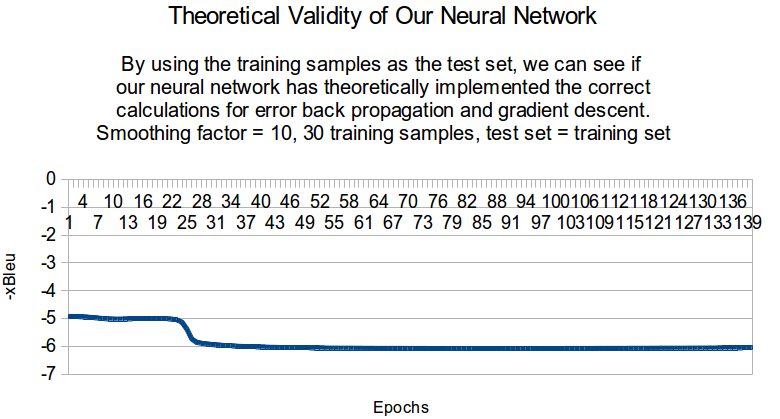
\includegraphics[width=\linewidth]{Theoretical_validity_graph}
\end{figure}

The second overnight experiment was conducted on a larger training set with 180 training samples and 20 test samples, this time using source sentences 1 to 180 from our input file \verb|test.input.tok.1| as training samples and sentences 181 to 200 as test samples. This choice of training samples means that the result are independent of the result in the first test, as none of the training samples overlap. Again, the result of our experiment suggest that the system works (see Figure \ref{training}), however after 14 epochs the gradients became very large and the system calculations outputted NaN again. Detailed system output can be found in the \verb|lcprtm/Result| directory and the results discussed in this section can be found in the \verb|lcprtm/Result/csv/| directory (also included in Appendix \ref{firstrun} and \ref{second}).

\begin{figure}
\label{training}
\caption{The results for second overnight experiment.}
\centering
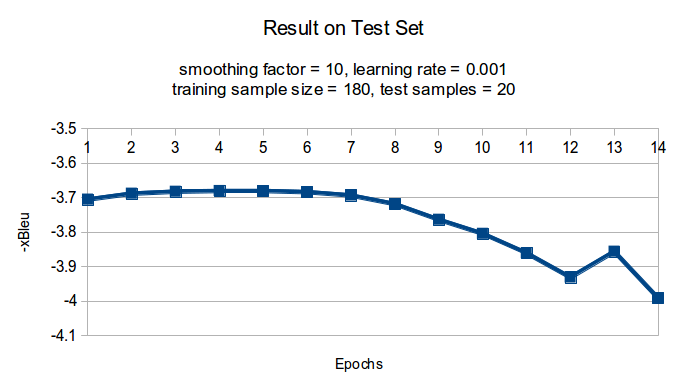
\includegraphics[width=\linewidth]{Smoothing10_200-training-samples_graph}
\end{figure}

\section{Conclusion}
We believe that our neural network correctly learns how to minimize the loss function $-xBleu$ and is relatively stable. Increasing \verb|smoothing_factor| will result in smaller gradients and slower training. Because we are getting NaN values (too big or too small numbers) after certain amounts of epochs with large training sets, we believe that \verb|smoothing_factor| should be increased for a more stable system. By how much can only be determined by trial and error, more experiments need to be conducted in order to tune the parameter \verb|smoothing_factor| in particular, and possibly \verb|learning_rate|. 

As of now, the training will run forever as we have not been able to tune the parameters for a sufficiently stable system in order to determine a good convergence criteria.

\bibliographystyle{plain}
\bibliography{Summary}

\pagebreak

\let\cleardoublepage\clearpage

\appendix

\section{Appendix}

\subsection{Results for first run}

\begin{table}[H]
\centering
\label{firstrun}
\caption{Results for first run.}
\begin{tabular}{|c|}%
\hline
\bfseries Loss function \\% specify table head
\hline
-3.705635097902438169 \\ \hline
-3.688438543285909699 \\ \hline
-3.682763400473420656 \\ \hline
-3.680557770067027779 \\ \hline
-3.680711280606880909 \\ \hline
-3.684001256719885653 \\ \hline
-3.693780268541727363 \\ \hline
-3.718753361569778981 \\ \hline
-3.763925242035965457 \\ \hline
-3.804602229567417560 \\ \hline
-3.860868119753573691 \\ \hline
-3.931406370914172221 \\ \hline
-3.856483504073254576 \\ \hline
-3.991880703457518997 \\
\hline
\end{tabular}
\end{table}

\subsection{Results for second run}

\begin{table}[H]
\label{second}
\caption{Results for second run.}
\begin{multicols}{3}
\begin{tabular}{|c|}%
\hline
\bfseries Loss function \\% specify table head
\hline
-4.925219768943486898 \\ \hline
-4.928882439772602098 \\ \hline
-4.934277387580417340 \\ \hline
-4.942461536588248272 \\ \hline
-4.953402019294050440 \\ \hline
-4.967205169862979552 \\ \hline
-4.983938877082958463 \\ \hline
-5.001246771383204504 \\ \hline
-5.014515411532945777 \\ \hline
-5.020956589315610508 \\ \hline
-5.021672773425295055 \\ \hline
-5.019218124702288009 \\ \hline
-5.015542066372502994 \\ \hline
-5.011747633699355831 \\ \hline
-5.008397666305318907 \\ \hline
-5.005783489490135629 \\ \hline
-5.004103627415170230 \\ \hline
-5.003577281610437133 \\ \hline
-5.004508825520574078 \\ \hline
-5.007374718842890537 \\ \hline
-5.013181137544878041 \\ \hline
-5.024749137618814032 \\ \hline
-5.051203953979976902 \\ \hline
-5.126880695576494062 \\ \hline
-5.377137947495798542 \\ \hline
-5.738500425794431870 \\ \hline
-5.858067110992541515 \\ \hline
-5.893931351373623784 \\ \hline
-5.917728160083535194 \\ \hline
-5.936434754999877939 \\ \hline
-5.951938120110934705 \\ \hline
-5.965122765282610651 \\ \hline
-5.976512393355510433 \\ \hline
-5.986458646403547412 \\ \hline
-5.995216147764370618 \\ \hline
-6.002978262580414004 \\ \hline
-6.009896557928029459 \\ \hline
-6.016092512769798617 \\ \hline
-6.021665115471935614 \\ \hline
-6.026696076217249676 \\ \hline
-6.031253554527745031 \\ \hline
-6.035394909507702188 \\ \hline
-6.039168778461275977 \\ \hline
-6.042616678100265482 \\ \hline
-6.045774257236814719 \\ \hline
-6.048672289554978043 \\ \hline
-6.051337469104096201 \\ \hline

\end{tabular}

\columnbreak

\begin{tabular}{|c|}%
\hline
\bfseries Loss function (2) \\% specify table head
\hline
-6.053793053843013361 \\ \hline
-6.056059390669773279 \\ \hline
-6.058154346998018802 \\ \hline
-6.060093667926703453 \\ \hline
-6.061891273652981305 \\ \hline
-6.063559508517056607 \\ \hline
-6.065109350617155393 \\ \hline
-6.066550589070367927 \\ \hline
-6.067891974564887825 \\ \hline
-6.069141347741340731 \\ \hline
-6.070305749074819346 \\ \hline
-6.071391513247576199 \\ \hline
-6.072404350461538591 \\ \hline
-6.073349416708183846 \\ \hline
-6.074231374666536176 \\ \hline
-6.075054446619877702 \\ \hline
-6.075822460554236137 \\ \hline
-6.076538890415599248 \\ \hline
-6.077206891350543927 \\ \hline
-6.077829330628897964 \\ \hline
-6.078408814842939378 \\ \hline
-6.078947713890874738 \\ \hline
-6.079448182179837623 \\ \hline
-6.079912177422676756 \\ \hline
-6.080341477351625556 \\ \hline
-6.080737694628298939 \\ \hline
-6.081102290192462512 \\ \hline
-6.081436585260475702 \\ \hline
-6.081741772156892267 \\ \hline
-6.082018924139373617 \\ \hline
-6.082269004356468223 \\ \hline
-6.082492874060158705 \\ \hline
-6.082691300179127403 \\ \hline
-6.082864962345139404 \\ \hline
-6.083014459452415146 \\ \hline
-6.083140315818993393 \\ \hline
-6.083242987009279901 \\ \hline
-6.083322865368059773 \\ \hline
-6.083380285308422231 \\ \hline
-6.083415528388702143 \\ \hline
-6.083428828207362749 \\ \hline
-6.083420375138604008 \\ \hline
-6.083390320926705286 \\ \hline
-6.083338783152148821 \\ \hline
-6.083265849578796569 \\ \hline
-6.083171582387856269 \\ \hline
\end{tabular}

\columnbreak

\begin{tabular}{|c|}%
\hline
\bfseries Loss function (3) \\% specify table head
\hline

-6.083056022301278176 \\ \hline
-6.082919192595031888 \\ \hline
-6.082761103000437153 \\ \hline
-6.082581753490504006 \\ \hline
-6.082381137947021621 \\ \hline
-6.082159247703573079 \\ \hline
-6.081916074959402785 \\ \hline
-6.081651616059136067 \\ \hline
-6.081365874633889668 \\ \hline
-6.081058864599810931 \\ \hline
-6.080730613011120944 \\ \hline
-6.080381162765855940 \\ \hline
-6.080010575163440123 \\ \hline
-6.079618932314816426 \\ \hline
-6.079206339406809434 \\ \hline
-6.078772926823822864 \\ \hline
-6.078318852131030958 \\ \hline
-6.077844301924228532 \\ \hline
-6.077349493552406834 \\ \hline
-6.076834676719656159 \\ \hline
-6.076300134973541489 \\ \hline
-6.075746187087095684 \\ \hline
-6.075173188341578268 \\ \hline
-6.074581531716643390 \\ \hline
-6.073971648993846451 \\ \hline
-6.073344011778441853 \\ \hline
-6.072699132443033498 \\ \hline
-6.072037564995075520 \\ \hline
-6.071359905868195739 \\ \hline
-6.070666794635203090 \\ \hline
-6.069958914638178271 \\ \hline
-6.069236993528223323 \\ \hline
-6.068501803704688058 \\ \hline
-6.067754162640379256 \\ \hline
-6.066994933076196084 \\ \hline
-6.066225023065030975 \\ \hline
-6.065445385841475634 \\ \hline
-6.064657019490308443 \\ \hline
-6.063860966383263218 \\ \hline
-6.063058312350388945 \\ \hline
-6.062250185548935910 \\ \hline
-6.061437754990152804 \\ \hline
-6.060622228681596724 \\ \hline
-6.059804851340848231 \\ \hline
-6.058986901635067035 \\ \hline
-6.058169688900330030 \\ \hline
-6.057354549295030033 \\ \hline
\end{tabular}

\end{multicols}

\end{table}


\end{document}

% [TOC]

% Learning Continuous Phrase Repesentations for Translation Modelling
% ===================================================================

% * __Authors:__ Kerry Zhang, Richard Luong
% * __Student-ID:__ 2014403073, 2014403075

% __Distribution of work between the authors__: To be sure that both of us made equal amount of work, the [pair programming](http://en.wikipedia.org/wiki/Pair_programming) technique was applied. 

% Description
% -----------

% Our project is to implement Phrase Embedding, as described in the paper by Gao et al [\[1\]](http://research.microsoft.com/pubs/211749/nn4smt.acl.v9.pdf).

% So when the system is trained, it will output a real number vector given a source sentence. For two similar sentence, the output differences should be smaller, than for two completely different ones.

% This is done by a neural network, with one hidden layer. The first layer has the same number of nodes as the vocabulary size of both lanugages. The second and the third layer is set to 100 nodes.

% The initialization of the weights of the first layer to the hidden layer, denoted as `W1`, is done by using a bilingual topic distribution, in this case solved by using Latent Dirchlet Allocation. The weights between the hidden layer and the third layer, `W2`, is an identity matrix.

% Optimization of the weights are done with [Stochastic gradient descent](http://en.wikipedia.org/wiki/Stochastic_gradient_descent). The training should be stopped according to early stop principle, as suggested in the paper, however we haven't fine tuned the system sufficiently to determine a stop condition as of yet.

% Dependencies
% ------------

% * python 2.7+
% * [NumPy](http://www.numpy.org/)
% * [Gensim](https://radimrehurek.com/gensim/index.html)

% How to run
% ----------

% Unzip the archive.

% Before the first run, `W1` needs to be initialized, using [Latent Dirchlet Allocation](http://en.wikipedia.org/wiki/Latent_Dirichlet_allocation).

% 	python preprocessing.py $corpus_source $corpus_target $n_best_list $reference_file

% where `$corpus_source` and `$corpus_target` are paths to the parallell corpuses the bilingual topic modelling should be based on, `$n_best_list` is a path to a list of the n best translation of source sentences and `$reference_file` is a path to the reference translation of those source sentences. Sentence-level BLEU score is also computed during this stage. The W1 initialization and BLEU score can be found in `data/weight_initialization.gz` and `sbleu.txt`

% After that the system should be trained with

% 	python main.py $source_sentence_file $n_best_list

% where `$source` is a path to the source sentences and `$n_best_list` is a path to the n best translation of these sentences.

% Output
% -------

% When the system converges, the weights of the neural network are written to the files `W1.gz` and `W2.gz`.


% Experiment Results and Discussion
% ----------

% After multiple overnight test runs of the system that resulted in calculations that outputted NaN due to calculations that accumulated into too large or small numbers, and other issues such as too big gradients resulting in a very unstable gradient descent, we finally managed to get a relatively stable system. The two main parameters that required tuning were: `learning_rate` and `smoothing_factor`, which can be altered at the top of `main.py`. See Equation 6 in the paper by Gao et. al. 2013 for an explanation of the smoothing factor.

% As of now, the most stable system we have produced came when the parameters were set as follows: `smoothing_factor = 10` and `learning_rate = 1000`. With these parameter values, we conducted two overnight test runs. 

% The first was to test the theoretical validity of our system, i.e. whether or not the implemented calculations of the gradients, as suggested by the paper, actually result in a lowering of the loss function defined as $-xBleu$. To do this, we used 30 training samples (sentence number 200 to 230 in the file `test.input.tok.1` provided by our teacher), performed the gradient descent training on the entire training set and then tested the new average $-xBleu$ score for the entire training set. I.e. we used the training set as our test set in order to test the theoretical validity of our neural network. The results (See Figure `lcprtm/Result/csv/Theoretical_validity_graph.png` ****INSERT GRAPH SOMEHOW???????????????*****) seem to suggest that the system is indeed performing a correct gradient descent.

% The second overnight experiment was conducted on a larger training set with 180 training samples and 20 test samples, this time using source sentences 1 to 180 from our input file `test.input.tok.1` as training samples and sentences 181 to 200 as test samples. This choice of training samples means that the result are independent of the result in the first test, as none of the training samples overlap. Again, the result of our experiment suggest that the system works (*******INSERT lcprtm/Result/csv/Smoothing10_200-training-samples_graph.png************), however after 14 epochs the gradients became very large and the system calculations outputted NaN again. Detailed system output can be found in the `lcprtm/Result` directory and the results discussed in this section can be found in the `lcprtm/Result/csv/` directory.

% ********
% TO DO:
% lcprtm/Result/csv innheåller de två sista overnight körningarna jag gjorde som typ confirm att systemet funkar någorlunda bra. Bifoga graferna på nåt sätt?
% ********

% Conclusion
% ----------
% We believe that our neural network correctly learns how to minimize the loss function $-xBleu$ and is relatively stable. Increasing `smoothing_factor` will result in smaller gradients and slower training. Because we are getting NaN values (too big or too small numbers) after certain amounts of epochs with large training sets, we believe that `smoothing_factor` should be increased for a more stable system. By how much can only be determined by trial and error, more experiments need to be conducted in order to tune the parameter `smoothing_factor` in particular, and possibly `learning_rate`. 

% As of now, the training will run forever as we have not been able to tune the parameters for a sufficiently stable system in order to determine a good convergence criteria.

% References
% ----------

% \[1\]: __Learning Continuous Phrase Representations for Translation Modeling__ by Gao et. al. 2013. 

